\documentclass[11pt]{article}

\usepackage{amsmath,amssymb,enumerate,algorithm,algorithmic,fullpage,graphicx}

\usepackage{setspace}
\onehalfspacing

% \everymath{\displaystyle}

\title{CS 221 Project Progress \\ Applying Varied Artificial Intelligence Techniques to Play 2048}
\author{Zhiyang He, Charles Lu, Stephen Ou \\ \texttt{\{hzyjerry,clu8,sdou\}@stanford.edu}}
\date{November 12th, 2015}

\begin{document}

\maketitle

\section{Introduction}

In this report, we will discuss our model for the game 2048 and the various algorithms (expectimax, minimax, alpha beta pruning) that we will use to play the game. We have also implemented the algorithms in Python and connected them to a front end website playing 2048. We will report the initial experimental results at the end.

\section{2048 model}

First, we would like to discuss how we model the game of 2048 into specific game states. For each game state, there are two things to keep track of: the board and the score. The board is a four by four matrix, and each cell contains an integer (that is a power of 2) that indicates the current value of that cell. 0 is used to indicate unoccupied cells. The score variable is used to keep track of all the points received so far. The rule of the game of 2048 states that score is incremented by the sum of the two tiles when two tiles with the same value get merged.

There are two main methods that are available through the 2048 game state: \texttt{getLegalActions()} and \texttt{generateSuccessor()}. We will describe each of them in details below.

\texttt{getLegalActions()}: If the current agent is the human, there are four possible moves. The human can swipe left, right, up, or down. There is one special case. A move is considered invalid if the board in the successor state is the same as the current state. For example, if the left three columns are all filled with tiles and they are have different values, swiping left is not a valid action because the successor state will not change. Next, if the current agent is the computer, there are maximum of sixteen possible moves. The computer can add a new tile with a value of 2 into an unoccupied cell.

\texttt{generateSuccessor()}: If the current agent is the human, all the tiles will slide in the direction specified. If the two neighboring tiles in that direction have the same value, they will collide and form a new tile with a new value that is the sum of the two old values. For example, if the board currently consists of only two tiles, both with a value of 2, at the bottom row. Swiping left will result in a merged tile with a value of 4, sitting in the bottom left corner. Next, if the current agent is the computer, a new tile with the value of 2 will be added at the specified cell given by the row and column number.

\section{Expectimax algorithm}

We use a similar version of the expectimax algorithm as the one presented in lecture. If the current agent is the human, we take the action that produces the maximum score from the recursion tree. If the current agent is the computer, we randomly pick one action (to be more specific, an unoccupied cell location). We will experiment with different depth values where the recursion stop and we use the evaluation functions explained below to provide an accurate numerical estimation of the current game state.

\section{Minimax algorithm}

We use a similar version of the minimax algorithm as the one presented in lecture. If the current agent is the human, we take the action that produces the maximum score from the recursion tree. If the current agent is the computer, we take the action (considering all possible insertions of new tiles) with the minimum score in the recursion tree. We will experiment with different depth values where the recursion stop and we use the evaluation functions explained below to provide an accurate numerical estimation of the current game state.

\section{Alpha beta pruning algorithm}

We use a similar version of the alpha beta pruning algorithm as the one presented in lecture. If the current agent is the human, we take the action that produces the maximum score from the recursion tree. However, if at any point as we loop through all the actions, the beta value is smaller or equal to the alpha value, we can terminate and return the maximum action so far. If the current agent is the computer, we take the action (considering all possible insertions of new tiles) with the minimum score in the recursion tree. Similarly, if at any point as we loop through all the actions the beta value is smaller or equal to the alpha value, we can terminate and return the minimum action so far. We will experiment with different depth values where the recursion stop and we use the evaluation functions explained below to provide an accurate numerical estimation of the current game state.

\section{A concrete example}

\begin{centering}

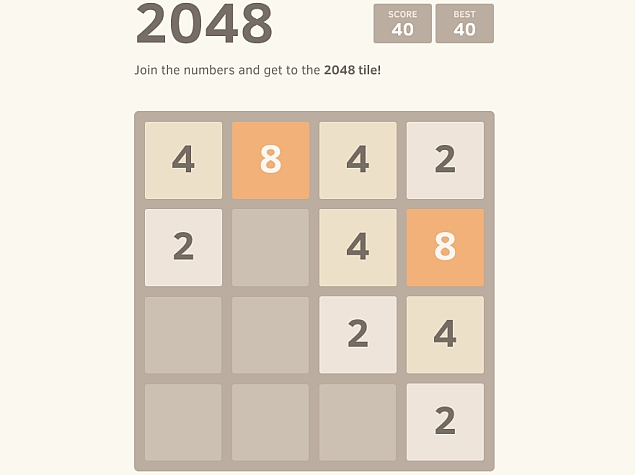
\includegraphics[width=90mm]{2048_screenshot.jpg}

\end{centering}

Say that we want to model the above state and run our algorithms. The board will be [[4, 8, 4, 2], [2, 0, 4, 8], [0, 0, 2, 4], [0, 0, 0, 2]]. The score will be 40. The legal actions are up, right, down, and left. Assume that we swipe down, the two 4 tiles on the third column will be merged. The new board will be [[0, 0, 0, 2], [0, 0, 0, 8], [4, 0, 8, 4], [2, 8, 2, 2]]. The new score will be 48 after incrementing by 8.

\section{Evaluation function}

With the framework for minimax and expectimax finished, the main task to improve their results is to provide a more accurate evaluation function. We have designed a number of evaluation functions of varying complexity to optimize for different purposes:

\begin{enumerate}[1)]

\item Exact score of a game state, based on the values on the game board

\item Slightly more complex evaluation function which weighs values in the top/left higher

\item Using a weighted combination of properties such as game score, smoothness (difference in values), monotonicity (ordering of tiles), and number of empty tiles

\item Very complex evaluation function based on advanced strategies:

\begin{enumerate}[i)]

\item Using a weighted sum of the board (similar to the second evaluation function), but treating the first and second columns as “storage” for multiple chains

\item Using similar metrics as in the second evaluation function

\item Penalizing moves which disrupt the consistency of the first two columns

\item Penalizing moves which put larger tiles in the second column

\item Adding weighted scores for the third and fourth columns depending on the maximum values in the first and second columns

\end{enumerate}

\end{enumerate}

\section{Training neural networks}

After experimenting with our designs of evaluation functions, we will use the implementation of expectimax/minimax and evaluation function which results in the highest mean score to train various models (with varying amounts of training/test data):

\begin{enumerate}[1)]

\item Simple linear classifiers

\item Neural networks with 1, 2, 3, etc. hidden layers with naive features

\item Linear classifiers and neural networks with additional heuristics

Using results on cross-validation data we will evaluate the performance (based on speed, mean score and variance, etc.) of the neural networks and compare to minimax and expectimax of varying depths.

\end{enumerate}

\section{Deep Q-learning}

Based on Google DeepMind’s deep Q-learning paper in \emph{Nature} [1], we have taken the implementation [2] and generalized it to accept an image (as pixels) and arbitrary heuristics as the reward for each move. The deep Q-learning module will be hooked into the front end to generate screenshots of the game state, rather than passing in the raw data. For features, we will be experimenting with the same models as we use for the neural networks. 

\section{2048 front end client}

In addition to our command line tool, we have forked the original 2048 repository to visualize the original 2048 game board in the browser. This will not only be used to visualize our minimax and expectimax algorithms with various evaluation functions, but also be used to generate screenshots of the game state for our deep Q-learning application. Based on the original 2048 repo, we have implemented \texttt{query\_server.py} to insert computer movements and \texttt{board.serialize()} to pass back actual states in the front end, including grid layout and current scores.

We use a lightweight Python web framework called Flask. On the front end, we send a HTTP request to an API endpoint with the board and the current score as parameters. The API endpoint in Flask will run the algorithm based on the board and the current score, and return an appropriate move. Corresponding simulation endpoint in Flask will receive the move and generate following game state. Meanwhile, the front end Javascript code will update visualization in the browser. 

\section{Preliminary experimental results}

First, we implement a randomized moving algorithm to test the basic performance of our simulator. At each step, a move is randomly chosen (up, right, down, left) and applied. For this task our simulator produces satisfying performance in executing the moves and visualizing results. Through multiple runs, our mean total score is 1082 and the standard deviation is 532. Most of the scores stays in the range of 900-1200, with the highest tile almost never going over 128. Occasionally the game terminates early with significantly lower score.

\begin{centering}

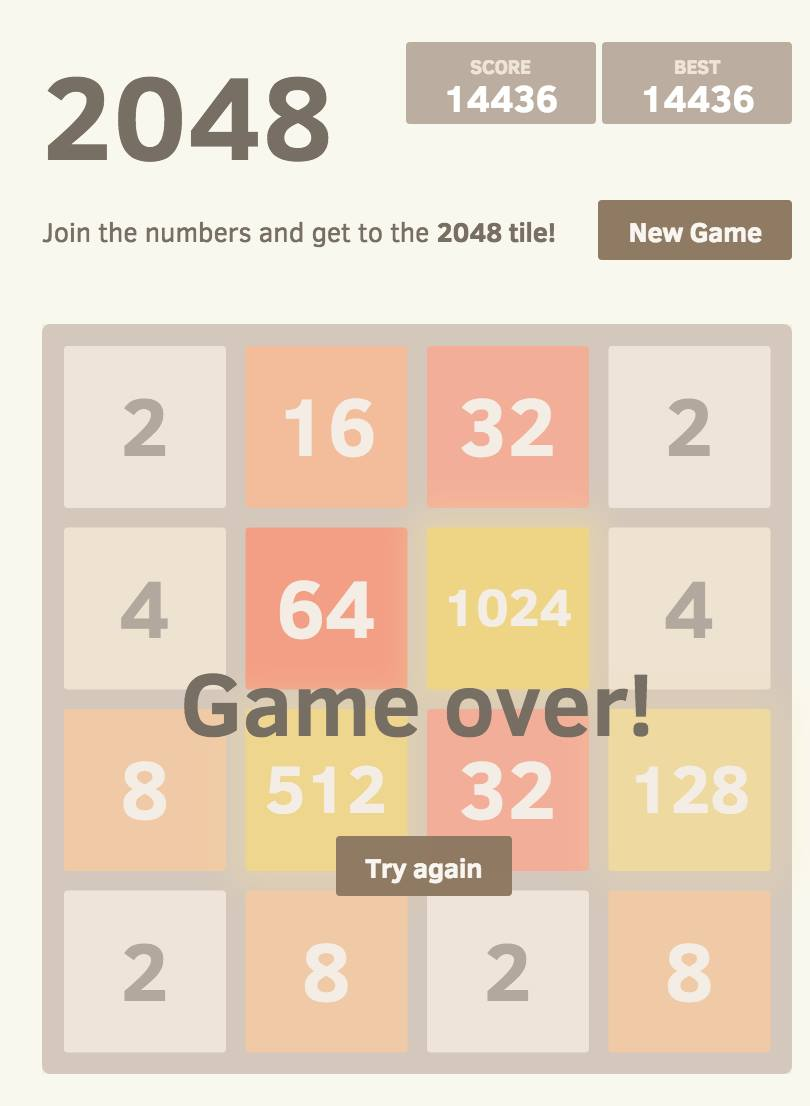
\includegraphics[width=90mm]{2048_screenshot2.jpg}

\end{centering}

With the working basic algorithm, we moved on to implementing a more advanced AI algorithm, the expectimax algorithm, mentioned above. We find out that even with limited search depth and an unrefined rudimentary evaluation function (only consider the current score), we are able to generate significantly better results than randomized movement. The highest tile goes beyond 1024 every time, and occasionally wins the game. The mean score through multiple runs is 5419 and the standard deviation is 1601.

\begin{thebibliography}{9}

\bibitem{1} \texttt{http://www.nature.com/nature/journal/v518/n7540/full/nature14236.html}

\bibitem{2} \texttt{https://sites.google.com/a/deepmind.com/dqn/}

\end{thebibliography}

\end{document}